\mychapter{5}{Signal extraction on DATA}
\label{sec:unchapitre}

In this section the results of the MVA training obtained in section 4 will be used to extract \textgamma+jet event
purity on real data via a maximum-likelihood fit.
The probability density function are determined on MC for the signal and sideband data for the background.
The analysis is performed on the $p_T^\gamma$ range [ 40 GeV ; 3000 GeV ] divided in 12 bins.
In each bin a fit is performed to the data distribution of the MVA to extract the number of signal and background event.

\section{Probability Density Function parametrization}

Maximum-likelihood fit is implemented using the ROOFit framework of ROOT.
Then the MVA response for data in the signal region is expressed as : 

\begin{equation}
F(MVA) = N_{signal}*f^{signal}(MVA) + N_{background}*f^{background}(MVA)
\end{equation}

With : 
\begin{itemize}
	\item $F(MVA) :=$ the MVA response for Data in the signal region.
	\item $f^{signal}(MVA) :=$ PDF for MC in the signal region.
	\item $f^{background}(MVA) :=$ PDF for Data in the sideband. 
	\item $N_{signal} :=$ number of signal events.
	\item $N_{background} :=$ number of background events. 
\end{itemize}

%\begin{figure}[h!]
%\centering
%    
\includegraphics[width=0.5\textwidth]{coming_soon}
%    \caption{Example of PDF parametrization for $p_T^\gamma \in [ 175 GeV ; 230 GeV ]$}
%    \label{coming_soon}
%\end{figure}

\section{Fit on Data}

With the PDF established in the previous section we want to extract values of the parameters $N_{signal}$ and $N_{background}$ representing
signal and background number of events in the sample. For this analysis we will perform a maximum-likelihood estimation for
each $p_T^\gamma$ range that has been defined. Fig. (\ref{pt_5_dataset}) show for example the fit perfomed for
$p_T^\gamma \in [ 175 GeV ; 230 GeV ]$

\begin{figure}[h!]
\centering
    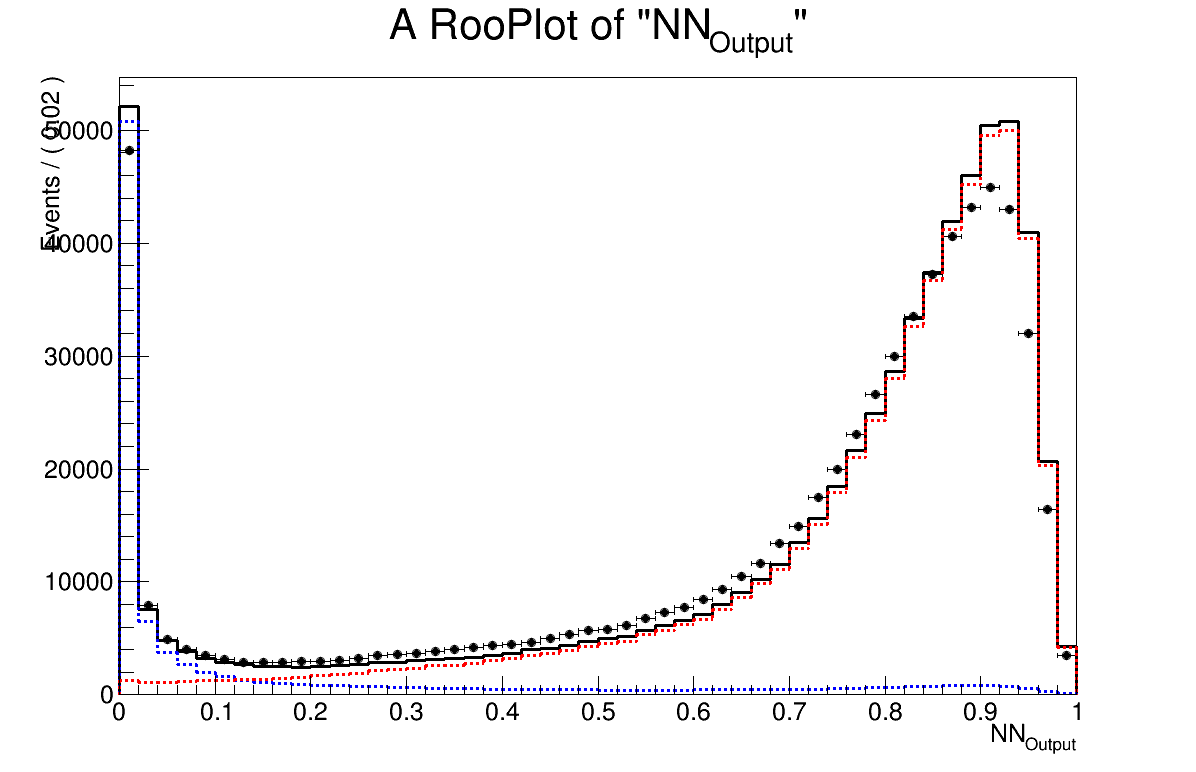
\includegraphics[width=0.7\textwidth]{pt_5_dataset}
    \caption{Example of a maximum likelihood fit performed for $p_T^\gamma \in [ 175 GeV ; 230 GeV ]$ on the ANN, showing background
    PDF (blue dotted line) signal PDF (red dotted line) and fit result (solid black line) superimposed with real data (black dot).}
    \label{pt_5_dataset}
\end{figure}

\subsection{Pulls distribution cross-check}

In order to validate the maximum-likelihood fit we generate a pull distribution for 
$10^4$ toyMC experiments for each $p_T^\gamma$ range. For each toyMC, a fake data sample is generated according to
$f^{signal}$, $f^{background}$, $N_{signal}$ and $N_{background}$.\\
The sample is then fitted with the same fit model to obtain $N^{fit}_{signal} \pm \sigma_{N_{signal}}$ and
$N^{fit}_{background} \pm \sigma_{N_{background}}$
To ensure the fit has no intrinsic bias, we look at the pull distribution defined as :

\begin{equation}
Pull = \frac{N^{fit}_{signal}-N^{generated}_{signal}}{\sigma^{fit}_{N_{signal}}}
\end{equation}

If the likelihood of the fitted variables is well described by a gaussian, we expect the mean of the pull distribution
to be centered with zero and its RMS to be centered with one.

\begin{figure}[h!]
\centering
    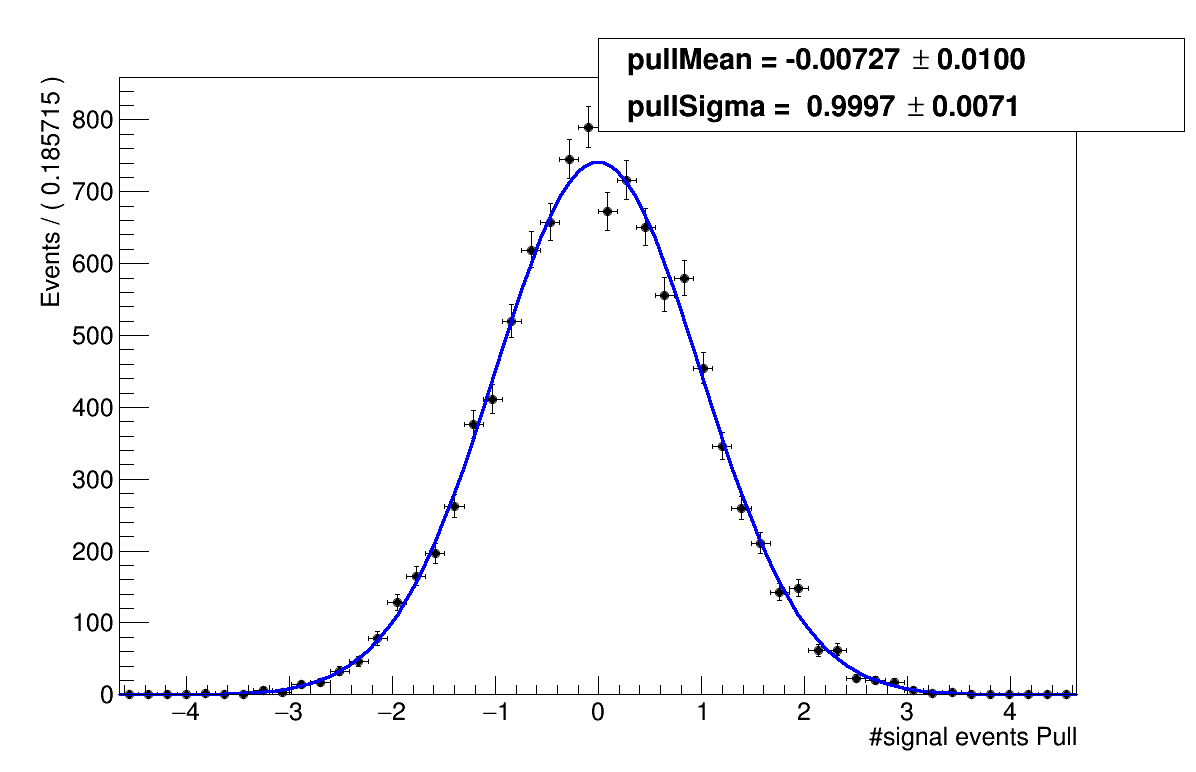
\includegraphics[width=0.7\textwidth]{pull_plot}
    \caption{Example of a pull plot performed for $p_T^\gamma \in [ 175 GeV ; 230 GeV ]$ with the ANN, showing pull
    results (black dot) and a gaussian fit (blue line)}
    \label{pull_plot}
\end{figure}

\subsection{\textgamma+jet events purity}

Finally the estimated number of signal and background events are used to construct the \textgamma+jet
events (signal) purity function of the $p_T^\gamma$ fig. (\ref{purity_bdt_ann}), defined as :

\begin{equation}
Purity = \frac{N_{signal}}{N_{signal}+N_{background}}
\end{equation}

We can see that the purity is at about 50\% at low $p_T^\gamma$ and goes up to 90\% around $p_T^\gamma$ ~ 500GeV. There
is a decreasing of the purity at 800 GeV, this could be due $p_T^\gamma$ dependance that hasn't been taken in account in the MVA's.

\begin{figure}[h!]
\centering
    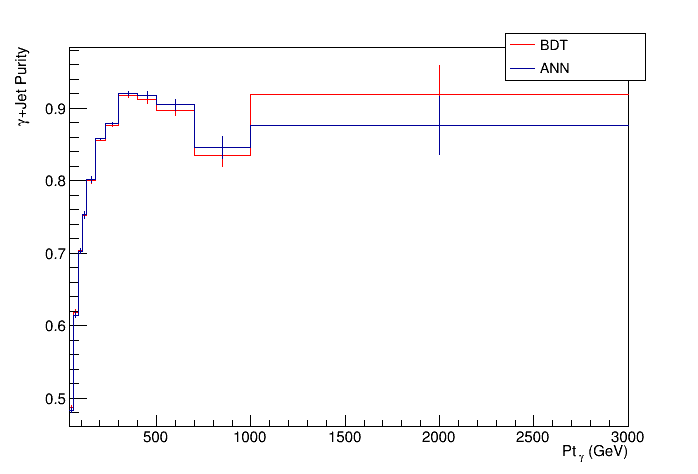
\includegraphics[width=0.7\textwidth]{purity_bdt_ann}
    \caption{\textgamma+jet purity function of $p_T^\gamma \in [ 40 GeV ; 3000 GeV ]$ evaluated with the BDT and the ANN.}
    \label{purity_bdt_ann}
\end{figure}

%%% Local Variables: 
%%% mode: latex
%%% TeX-master: "isae-report-template"
%%% End: 
